% Digital Logic Report Template
% Created: 2019-09-13, John Miller

%==========================================================
%=========== Document Setup  ==============================

% Formatting defined by class file
\documentclass[11pt]{article}

% ---- Document formatting ----
\usepackage[margin=1in]{geometry}	% Narrower margins
\usepackage{booktabs}				% Nice formatting of tables
\usepackage{graphicx}				% Ability to include graphics

%\setlength\parindent{0pt}	% Do not indent first line of paragraphs 
\usepackage[parfill]{parskip}		% Line space b/w paragraphs
%	parfill option prevents last line of pgrph from being fully justified

% Parskip package adds too much space around titles, fix with this
\RequirePackage{titlesec}
\titlespacing\section{0pt}{8pt plus 4pt minus 2pt}{3pt plus 2pt minus 2pt}
\titlespacing\subsection{0pt}{4pt plus 4pt minus 2pt}{-2pt plus 2pt minus 2pt}
\titlespacing\subsubsection{0pt}{2pt plus 4pt minus 2pt}{-6pt plus 2pt minus 2pt}

% ---- Hyperlinks ----
\usepackage[colorlinks=true,urlcolor=blue]{hyperref}	% For URL's. Automatically links internal references.

% ---- Code listings ----
\usepackage{listings} 					% Nice code layout and inclusion
\usepackage[usenames,dvipsnames]{xcolor}	% Colors (needs to be defined before using colors)

% Define custom colors for listings
\definecolor{listinggray}{gray}{0.98}		% Listings background color
\definecolor{rulegray}{gray}{0.7}			% Listings rule/frame color

% Style for Verilog
\lstdefinestyle{Verilog}{
	language=Verilog,					% Verilog
	backgroundcolor=\color{listinggray},	% light gray background
	rulecolor=\color{blue}, 			% blue frame lines
	frame=tb,							% lines above & below
	linewidth=\columnwidth, 			% set line width
	basicstyle=\small\ttfamily,	% basic font style that is used for the code	
	breaklines=true, 					% allow breaking across columns/pages
	tabsize=3,							% set tab size
	commentstyle=\color{gray},	% comments in italic 
	stringstyle=\upshape,				% strings are printed in normal font
	showspaces=false,					% don't underscore spaces
}

% How to use: \Verilog[listing_options]{file}
\newcommand{\Verilog}[2][]{%
	\lstinputlisting[style=Verilog,#1]{#2}
}




%======================================================
%=========== Body  ====================================
\begin{document}

\title{ELC 2137 LaTeX Tutorial}
\author{John Miller}
\maketitle


\section*{Overview}
TeX is a computer language for typesetting or formatting documents created by Donald Knuth in the 1970s.  It was expanded by Leslie Lamport in the 1980s, and others since then, to create LaTeX (pronounced ``lay-tek'' or ``lah-tek''). TeX is actually Greek ``tau epsilon chi'' $\tau \epsilon \chi$, related to our word ``technology.''  For more, see \href{https://en.wikipedia.org/wiki/LaTeX}{Wikipedia: LaTeX} or \href{http://tug.org/whatis.html}{History of TeX}.

It is designed for the author to focus more on the content and less on the formatting, allowing the compiler to take care of it.  However, this can be difficult for people who have grown up with WYSIWYG (what you see is what you get) editors like Microsoft Word and PowerPoint.  

Recommendation: Work \textit{with} the tools to create great reports, not \textit{against} them.


\section*{Getting Started}

The ECS lab computers already have MikTeX (compiler) and TeXstudio (editor) installed.  MikTeX comes with its own editor (TeXworks), but it's very basic and not as easy to use as TeXstudio.  If you want to install them on your personal computer, here are the links:

\begin{itemize}
	\item \url{https://miktex.org/}
	\item \url{http://texstudio.sourceforge.net/}
\end{itemize}

If you get stuck, you can find the answer to almost any question by searching the internet for ``latex \{your question\}''.  For example, try ``latex figures''.  Here are some good references if you need them:

\begin{itemize}
	\item \url{https://www.latex-tutorial.com/tutorials/}
	\item \url{https://en.wikibooks.org/wiki/LaTeX}
\end{itemize}


\section*{Sections}

You'll notice that this document is broken into sections with headings.  This is accomplished with the commands \verb|\section*{}, \subsection*{}, \subsubsection*{}|.  The heading text is placed inside the braces.  Without the `*', the headings have numbers, like ``1.4 Title''.



\section*{Text Formatting \& Environments}
% Note: the star (*) removes the number

Text can be formatted with some simple commands, such as:

\begin{itemize}
	\item \verb|\textbf{bold}| = \textbf{bold}
	\item \verb|\textit{italic}| = \textit{italic}
	\item \verb|\texttt{typewriter}| = \texttt{typewriter} (mono-spaced)
	\item \verb|\_| and \verb|\&| and \verb|\#| = \_ (underscore) and \& and \#
\end{itemize}

\subsection*{Lists}

The bulleted list above is an \texttt{itemize} environment.  Similar, the \texttt{enumerate} environment creates a numbered list, like:

\begin{enumerate}
	\item Here is an item.
	\item Here is another.
	\item The last one.
\end{enumerate}

You can also nest lists, like this:

\begin{enumerate}
	\item Colors
	\begin{enumerate}
		\item Red
		\item Green
		\item Blue
	\end{enumerate}
	\item People
	\item Places
\end{enumerate}

or this:

\begin{itemize}
	\item Colors
	\item People
	\item Places
		\begin{itemize}
		\item Waco
			\begin{itemize}
			\item Rogers ECS Building
			\item McLane Stadium
			\end{itemize}
		\item DFW
		\item Houston
		\end{itemize}
\end{itemize}



\subsection*{Center Align}

Another useful environment is \texttt{center}.  This aligns whatever content is inside of it in the center of the body.

\begin{center}
	This sentence is centered.
\end{center}


\section*{Tables and Figures - Not floating}

Tables and images (figures) are typically ``floating'' objects, which is explained in the next section.  However, they can be included directly with just a few commands.  The advantage of this method is you get them exactly where you want them.

We use the \texttt{tabular} environment to define a table:

\begin{tabular}{cc|c}
	\toprule
	A & B & AND \\
	\midrule
	0 & 0 & 0 \\
	0 & 1 & 0 \\
	1 & 0 & 0 \\
	1 & 1 & 1 \\
	\bottomrule
\end{tabular} 

If you want it centered, you can put it inside a \texttt{center} environment:

\begin{center}
	\begin{tabular}{cc|c}
		\toprule
		A & B & AND \\
		\midrule
		0 & 0 & 0 \\
		0 & 1 & 0 \\
		1 & 0 & 0 \\
		1 & 1 & 1 \\
		\bottomrule
	\end{tabular} 
\end{center}

You can include an image using the \verb|\includegraphics| command:

\begin{center}
	
\includegraphics[width=0.5\textwidth]{BUlogo}
\end{center}

You can even put it in the middle 
\includegraphics[width=0.1\textwidth]{BUlogo}
of a sentence if you want. The \verb|\includegraphics| command is explained in detail below.

If you need to include a full-page PDF or something of that sort, this might be a good way to do it:

% Use quotes (" ") for files with spaces in the name


\section*{Tables and Figures - Floating}

Tables and figures are intended to be ``floating'' objects, meaning LaTeX will move them around to make them best fit the flow of the document.  You may not think so, but there is a method to what might seem like madness. One of the main reasons to use these environments is that you can provide a caption and reference them in the body, as in: 

Table \ref{tbl:example_table} is an example of a truth table. The full logo is shown in Figure \ref{fig:original_logo}, while Figure \ref{fig:another_image} shows how to crop it.


\begin{table}[ht]\centering
	\caption{Example of a floating table}
	\label{tbl:example_table}
	\begin{tabular}{cc|c}
		\toprule
		A & B & AND \\
		\midrule
		0 & 0 & 0 \\
		0 & 1 & 0 \\
		1 & 0 & 0 \\
		1 & 1 & 1 \\
		\bottomrule
	\end{tabular} 
\end{table}

Captions are important for figures and tables.  Typically, they should be above a table and below a figure. Labels provide a way to reference a particular figure or table. Note: The label must come \textbf{after} the caption.  
%This paragraph is supposed to be after the table and before the figures.

The \verb|\includegraphics| command has lots of options.  Here are a few that you might find useful:  (note: \texttt{\#} = a number you need to fill in)

\begin{center}
	\begin{tabular}{ll}
		Adjust size:      		& \texttt{height=\#} (length) \\
								& \texttt{width=\#} (length) \\
								& \texttt{scale=\#} (0 to 1) \\
		Rotate:  				& \texttt{angle=\#} (degrees) \\
		Cropping:  				& \texttt{trim=\# \# \# \#} (order is: left bottom right top) \\
								& \texttt{clip} (this removes what you just trimmed) \\
		Choose page of a pdf: 	& \texttt{page=\#} \\
	\end{tabular}
\end{center}

(Note: The above list is actually a \verb|tabular| environment, just without any border lines.)

Here are a few examples:

Figure \ref{fig:original_logo} uses the command: \verb|
\includegraphics[width=0.5\textwidth]{BUlogo}|.  The \texttt{width} option scales the whole image to be half of the width of a line of text (using the built-in length command \verb|\textwidth|).

\begin{verbatim}
\begin{figure}[ht]\centering
    
\includegraphics[width=0.5\textwidth]{BUlogo}
    \caption{This is the original logo.}
    \label{fig:original_logo}
\end{figure}
\end{verbatim}

\begin{figure}[ht]\centering
	
\includegraphics[width=0.5\textwidth]{BUlogo}
	\caption{This is the original logo.}
	\label{fig:original_logo}			% label must be after caption
\end{figure}

This sentence is supposed to be between the figures.

\begin{figure}[ht]\centering
	
\includegraphics[width=0.5\textwidth,trim=0cm 5cm 0cm 5cm,clip]{BUlogo}
	\caption{This is the logo cropping the top and bottom.}
	\label{fig:another_image}		% label must be after caption
\end{figure}

% Uncomment this line to see an example of the \clearpage command
%\clearpage

This paragraph comes after both figures. If there is enough text here, LaTeX will put it on the same page as the figures, pushing them to the top.  More text. More text. More text. More text. More text. More text. More text. More text. More text. More text. More text. More text. More text.

You can use the \verb|\clearpage| command to force all floats that have been defined so far to be drawn and then start the next line on a new page.  See an example by uncommenting the command in the .tex file of this document.


\section*{Code}
There is a LaTeX add-on package called ``listings'' that allows you to easily include code from lots of different languages, including Verilog.  At the top of this .tex document, you'll notice some commands for setting up the listings package and ``macros'' or user-defined commands that make it even easier.  There are two ways to include code.  You will probably want to use the first one, which reads directly from your code file.  

\subsection*{File Inclusion}

\Verilog[caption=File-included Verilog code example,label=code:file_ex]{example_or.sv}

You can also include only specific lines.

\Verilog[firstline=6, lastline=7, caption=Selected lines from example file,
label=code:file_ex_lines]{example_or.sv}

The only downside to this is that you have to tell LaTeX where your file is relative to the location of your LaTeX file.  For example, suppose you have a file structure like this:

\texttt{%
\hspace*{5ex}BaseFolder \\
	\hspace*{10ex}Folder1 \\
		\hspace*{15ex}report.tex ~~~~~~ <-- LaTeX file\\
		\hspace*{15ex}code1.sv \\
		\hspace*{15ex}SubfolderA \\
			\hspace*{20ex}figureA.png \\
			\hspace*{20ex}codeA.sv \\
		\hspace*{15ex}SubfolderB \\
	\hspace*{10ex}Folder2 \\	
		\hspace*{15ex}figure2.jpg \\
		\hspace*{15ex}code2.sv 
}

To include \texttt{code1.sv}, which is in the same folder as the LaTeX file, you would use the command:\\
\hspace*{5ex}\verb|\Verilog{code1.sv}|

To include \texttt{codeA.sv}, you would use the command:\\
\hspace*{5ex}\verb|\Verilog{SubfolderA/codeA.sv}|

To include \texttt{code2.sv}, you would use the command:\\
\hspace*{5ex}\verb|\Verilog{../Folder2/code2.sv}|

This one is a little trickier to understand.  The ``\texttt{..}'' tells the compiler to go ``up'' or ``out'' one folder level.  Thus, it starts at \texttt{BaseFolder} and then follows the remaining steps (\texttt{BaseFolder -> Folder2 -> code2.sv}).  

Note: You can do multiple of these, as in \texttt{../../../folder/folder/file}, but it gets confusing pretty fast.  This is one reason why we require you to use the folder structure we do.

\subsection*{Direct Inclusion}

The other way to include code is to copy and paste it directly into the LaTeX document inside of a \texttt{lstlisting} (pronounced ``list-listing'') environment, like this:

\begin{lstlisting}[style=Verilog,
caption=Direct Verilog code example,
label=code:ex 
]
module example_and(
	input a, b,
	output c
	);
	
	// c = a AND b
	and(c,a,b);	
endmodule
\end{lstlisting}

Notice that the format of the output (in the PDF) is exactly the same.


\section*{Equations}
We will not write a lot of equations in 2137.  It is included here for completeness and because this is another thing at which LaTeX excels.  There are different equation environments.  I'll only cover the most basic one here, which is the ``in-line'' version that uses single dollar signs, like this:

The equation for electrical power is $P = VI$.  When delivering power to a resistor, where $V = RI$, this can written as $P = VI = RI^2 = \frac{V^2}{R}$.

For more, see
\begin{itemize}
	\item \url{https://www.latex-tutorial.com/tutorials/amsmath/}
	\item \url{https://en.wikibooks.org/wiki/LaTeX/Mathematics}
\end{itemize}



\section*{Report Items}

\subsection*{Report Format}
Unless otherwise specified in the assignment, each report will have the same format: Summary, Results, and Code. 
\begin{itemize}
	\item In the Summary section, you should provide a brief overview of the purpose of the lab and summarize your results. 
	\item In the Q\&A section, answer any questions posed in the assignment.  Alternatively, your instructor might want you to include these in your summary.
	\item The Results section will include your simulation waveforms, results tables, pictures of hardware, and any other required items.  
	\item The Code section includes all of the files you wrote or modified as part of the lab.  Provided files that you did not change do not need to be included here.
\end{itemize}

\subsection*{Q\&A Formatting}
One way to nicely format your responses to questions is the following:

\begin{enumerate}
	\item How should I format them?
	
	Use the same numbered list format as in the assignment (like this).
	
	\item Do I need to include the original question?
	
	Yes, include both the question and the answer to it.
	
	\item Should I put the question on the first line?
	
	Yes, then skip a line and write your answer.  This produces a nicely formatted result.
\end{enumerate}


\subsection*{Simulation Results}
You will include screen captures of simulation waveforms from Vivado.  The easiest way to do this is to use the Windows Snipping Tool or Snip \& Sketch.  Use Rectangular mode and select only the relevant part of the simulation window, then save it as a PNG image.  You will notice that on Figure \ref{fig:sim_with_table} you can read the signal names on the left, see the time values across the top, and see all of the signal values up to the stop time of 40 ns. 

Note: By default, the background in Vivado is black. If you were going to print your report, we would require you to change it (to save ink).  But since we are going to grade everything electronically, it doesn't matter.


\subsection*{Expected Results Table}
For each simulation you run, you need to create an ``expected results table'' (ERT).  This table should show what values are expected for each input and output signal at each time step of the simulation.  Always position your table above the simulation waveform, as done with Figure \ref{fig:sim_with_table}.  Putting the \texttt{tabular} environment inside of the \texttt{figure} environment ensures that the table and waveform won't be separated by a page break.  Note: you can use this example as a template.

\begin{figure}[ht]\centering
	\begin{tabular}{l|rrrr}
		Time (ns): & 0 & 10 & 20 & 30 \\
		\midrule
		a & 0 & 1 & 0 & 1 \\
		b & 0 & 0 & 1 & 1 \\
		\midrule
		c & 0 & 0 & 0 & 1 \\
		s & 0 & 1 & 1 & 0 \\
		\bottomrule
	\end{tabular}\medskip
	
	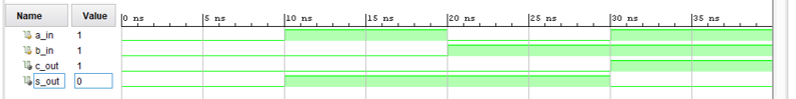
\includegraphics{sim_waveform}
	\caption{Example of a simulation waveform and ERT}
	\label{fig:sim_with_table}
\end{figure}


\section*{TeXstudio Shortcuts}
Some keyboard shortcuts you might find useful:

\begin{itemize}
	\item F5 -- compile to PDF
	\item Starting typing a command, then use arrows to choose the desired auto-complete command, and press Enter.  For example, type \verb|\V| and the first item in the pop-up list should be the \verb|\Verilog| command.
	\item In tables, TeXstudio will highlight things in red when the number of columns specified doesn't match the number of columns you have in a particular row.  Summary: When nothing is red, you have the right number everywhere!
	\item Text formatting, similar to MS Word:
	\begin{itemize}
		\item Ctrl+b = \textbf{bold}
		\item Ctrl+i = \textit{italic}
		\item Ctrl+Shift+t = \texttt{typewritter (monospaced)}
	\end{itemize}
	\item Ctrl+Shift+i = insert ``\verb|\item |''
	\item Standard Windows shortcuts:
	\begin{itemize}
		\item Ctrl+z = undo
		\item Ctrl+y = redo
		\item Ctrl+c = copy
		\item Ctrl+x = cut
		\item Ctrl+v = paste
	\end{itemize}
\end{itemize}




\end{document}
